\section{Clean Architecture}
\label{ca:sec:clean_architecture}

\begin{itemize}
	\item \textbf{Dependency Direction}:
	\begin{itemize}
		\item \itquote{Depend in the direction of stability.}
		\item Flüchtige Komponenten sollten sich nicht auf schwer änderbare Komponenten verlassen
	\end{itemize}
	\item \textbf{Clean Architecture Style}:
	\begin{itemize}
		\item Konzentrische Kreise, je näher dem Zentrum desto mehr \quotestyle{high-level}
		\item Äußere Kreise beschreiben \textbf{Mechanismen}, innere \textbf{Policies}
		\item \textbf{Dependency Rule}: Dependencies zeigen immer nach innen
		\item Interaktion zwischen Layern durch \textbf{Adapter-Klassen}
	\end{itemize}
	\item \textbf{Vorteile}:
	\begin{itemize}
		\item Verbesserte Testbarkeit
		\item \textbf{Unabhängigkeit} von Frameworks, UI, Datenbanken oder der Außenwelt
	\end{itemize}
\end{itemize}

\begin{figure}[!h]
	\centering
	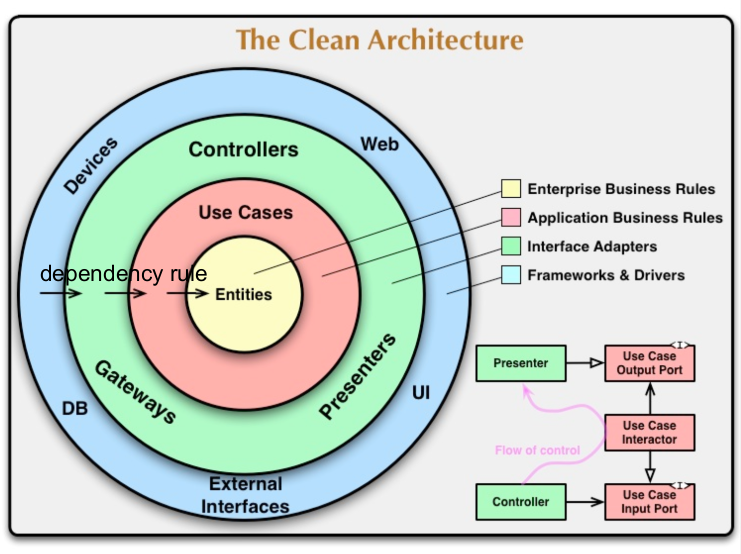
\includegraphics[width=0.85\textwidth]{images/clean_architecture.png}
\end{figure}